% =====================================================================
\chapter{Primer instrumento: el corpus de noticias}
\chaptermark{El corpus de noticias}
\label{cap:corpus}

Para medir el tono de la prensa económica primero hay que tenerla. No existe un archivo
público y ordenado de las notas de economía de los portales argentinos, así que el corpus se
construyó con \textit{web scraping}: la extracción automática de información de páginas web.
Este capítulo describe cómo se recolectó, cómo se auditó y cómo se ordenó cada nota en el
tiempo del mercado.

% ---------------------------------------------------------------------
\section{Recolección}
\label{sec:recoleccion}

Para un corpus histórico de noticias hay dos caminos, y se usaron los dos según la
disponibilidad de cada portal:

\begin{itemize}
  \item \textbf{Internet Archive.} Su \textit{Wayback Machine} guarda capturas de millones de
        páginas, y su API CDX permite listar las capturas de un sitio en un rango de fechas.
        Así se puede reconstruir una ventana más larga que la que exponen los propios portales,
        a costa de depender de qué capturó un tercero \citep{garg2025wayback}. Se usó para
        Ámbito Financiero (Economía y Finanzas), Clarín (Economía), Infobae, La Nación y TN.
  \item \textbf{Mapas del sitio.} Los portales publican archivos \texttt{sitemap.xml} para los
        buscadores, que listan sus notas recientes. Se usaron para Clarín, El Economista e
        iProfesional. Clarín se cubrió con ambos métodos: la ventana más profunda por la
        Wayback Machine y las notas más recientes por el mapa del sitio.
\end{itemize}

Una vez obtenida la página, hay que separar el texto de la nota del «relleno» (menús,
publicidad, firmas) y extraer sus metadatos. Se usó una estrategia en capas: los datos
estructurados JSON-LD primero, después las metaetiquetas Open Graph, el título
\texttt{<h1>}, la librería \texttt{trafilatura} \citep{barbaresi2021} y, como último recurso,
reglas sobre el HTML con BeautifulSoup. Cada nota se guardó con su sitio, fecha y hora de
publicación, título, bajada, contenido y etiquetas. El acceso autenticado a la API de Internet
Archive usa credenciales guardadas en un archivo de configuración externo, fuera del código.

El corpus final tiene \textbf{14.012 artículos} de siete portales, recolectados en nueve
fuentes (tabla~\ref{tab:corpus}): unos 63 millones de caracteres, alrededor de 4.500 por
artículo. Aunque abarca de enero de 2025 a mayo de 2026, en la práctica empieza en mayo de
2025: 14.001 de las 14.012 notas son del 1 de mayo de 2025 en adelante, porque tanto la
retención de los mapas del sitio como las capturas de la Wayback Machine se concentran en los
meses más recientes.

\begin{table}[H]
\centering\small
\begin{tabular}{@{}llr@{}}
\toprule
\textbf{Portal} & \textbf{Método de recolección} & \textbf{Artículos} \\
\midrule
iProfesional & Mapa del sitio & 5.455 \\
Clarín & Mapa del sitio & 3.737 \\
Clarín — Economía & Wayback Machine & 294 \\
El Economista & Mapa del sitio & 2.695 \\
Ámbito Financiero — Economía & Wayback Machine & 498 \\
Ámbito Financiero — Finanzas & Wayback Machine & 240 \\
Infobae — Economía & Wayback Machine & 500 \\
La Nación — Economía & Wayback Machine & 491 \\
TN — Economía & Wayback Machine & 102 \\
\midrule
\textbf{Total} & & \textbf{14.012} \\
\bottomrule
\end{tabular}
\caption{Corpus de noticias por fuente, después de la depuración. Fuente: elaboración propia
(\carpeta{Lado Noticias/noticias}).}
\label{tab:corpus}
\end{table}

% ---------------------------------------------------------------------
\section{Auditoría y depuración}

Las herramientas de extracción de contenido fallan con frecuencia en el relleno y en los
metadatos \citep{foley2026wcxb}, por lo que un corpus web tiene que auditarse antes de usarse:
buscar plantillas, duplicados y contenido que no corresponde \citep{dodge2021c4}. Los
duplicados, además, distorsionan cualquier modelo que se entrene con ese texto
\citep{lee2021dedup}. La auditoría encontró cinco problemas, cada uno con su solución
(tabla~\ref{tab:depuracion}).

\begin{table}[H]
\centering\small
\begin{tabularx}{\linewidth}{@{}L{3.4cm}YY@{}}
\toprule
\textbf{Problema} & \textbf{Qué se encontró} & \textbf{Solución} \\
\midrule
Duplicados exactos & 205 notas de Clarín descargadas dos veces, por Wayback Machine y por el mapa del sitio & Una copia por URL (la del sitio); los recolectores verifican la URL contra todo el corpus \\
Publicación cruzada & 208 grupos de título repetido; 175 se descartaron por estar a más de 48 horas (columnas recurrentes) & Los 33 grupos restantes (68 notas) se verificaron con Qwen3: 14 republicaciones reales \\
Metadatos faltantes & Sin autor ni palabras clave en iProfesional y sin fecha en 194 notas de El Economista, por un error de parseo del JSON-LD & Parseo tolerante; 192 notas reales se volvieron a descargar y recuperaron su fecha \\
Contenido que no es noticia & 2 páginas índice, 9 páginas de suscripción y 6 notas fuera de la ventana (fechadas por su última modificación) & Se eliminaron; los recolectores filtran por fecha de publicación efectiva \\
Plantillas & 65 grupos (479 notas) con el mismo comienzo; cuatro plantillas de El Economista concentran 325 notas con sentimiento constante & Se eliminaron 419 notas (2,9\%): el corpus pasó de 14.431 a 14.012 \\
\bottomrule
\end{tabularx}
\caption{Problemas del corpus y cómo se resolvieron. Fuente: elaboración propia a partir de
la auditoría del lado de noticias (\carpeta{Lado Noticias/noticias}).}
\label{tab:depuracion}
\end{table}

Las plantillas merecen un comentario, porque muestran por qué la auditoría es parte del
instrumento y no un trámite. Notas como el reporte diario «Dólar hoy» tienen fecha y
cotizaciones propias, pero el modelo de sentimiento les asignaba siempre el mismo valor, con
desvío cero entre decenas de notas: el valor dependía de la parte fija del texto y no de la
información del día. Replicado durante meses, ese valor sesgaba el promedio diario. En los
grupos de menos de 11 notas se conservó la más antigua (83 eliminadas); en los de 11 o más,
cuyo cuerpo es relleno, se eliminaron todas (336). Una sola nota de 2014 mal fechada, además,
estiraba la serie diaria a 4.186 días; tras la depuración la serie abarca 487 días. La
verificación de duplicados semánticos se hizo con el modelo de lenguaje abierto Qwen3, servido
localmente con Ollama.

% ---------------------------------------------------------------------
\section{Cada nota a su rueda}
\label{sec:alineacion}

Las noticias se publican a cualquier hora, pero el precio se forma solo en las ruedas, de lunes
a viernes de 11:00 a 17:00. Para medir si una nota mueve el precio hay que compararla con el
primer precio que pudo verse afectado por ella: una nota del martes a las 20:00 sale con el
mercado cerrado, y la primera vez que alguien puede operar con esa información es el miércoles.
Se aplicó la siguiente regla:

\begin{itemize}
  \item Todas las horas se pasaron a hora argentina: Clarín, Infobae y La Nación informan la
        hora en UTC, y 95 notas nocturnas cambian de fecha con la conversión.
  \item Una nota publicada antes de las 17:00 de un día con rueda cuenta para esa rueda.
  \item Una nota publicada a las 17:00 o después cuenta para la rueda siguiente.
  \item Una nota publicada en un día sin rueda (fin de semana o feriado) cuenta para la
        primera rueda posterior.
\end{itemize}

Dentro de la ventana común con el mercado (05/05/2025 al 30/04/2026, 244 ruedas) quedaron
13.925 notas (tabla~\ref{tab:alineacion}); las 10 de enero a marzo de 2025 y las 77 del cierre
del 30/04/2026 en adelante quedan afuera. Las 244 ruedas reciben noticias: mínimo 12, mediana 55
y máximo 145. Los lunes reciben el fin de semana: mediana de 85 notas, contra 50 el resto de los
días (figura~\ref{fig:u1}).

\begin{table}[H]
\centering\small
\begin{tabular}{@{}lrr@{}}
\toprule
\textbf{Dónde quedó cada nota} & \textbf{Notas} & \textbf{\%} \\
\midrule
En su mismo día (antes de las 17:00 de un día con rueda) & 8.332 & 59,8 \\
En la rueda siguiente, por salir después del cierre & 3.451 & 24,8 \\
En la rueda siguiente, por salir en un día sin rueda & 2.142 & 15,4 \\
\midrule
Total dentro de la ventana & 13.925 & 100,0 \\
\bottomrule
\end{tabular}
\caption{Asignación de las notas a las ruedas con la regla de las 17:00. Fuente: elaboración
propia (\carpeta{Unión/01_alineacion_noticias_ruedas}).}
\label{tab:alineacion}
\end{table}

\begin{figure}[H]
\centering
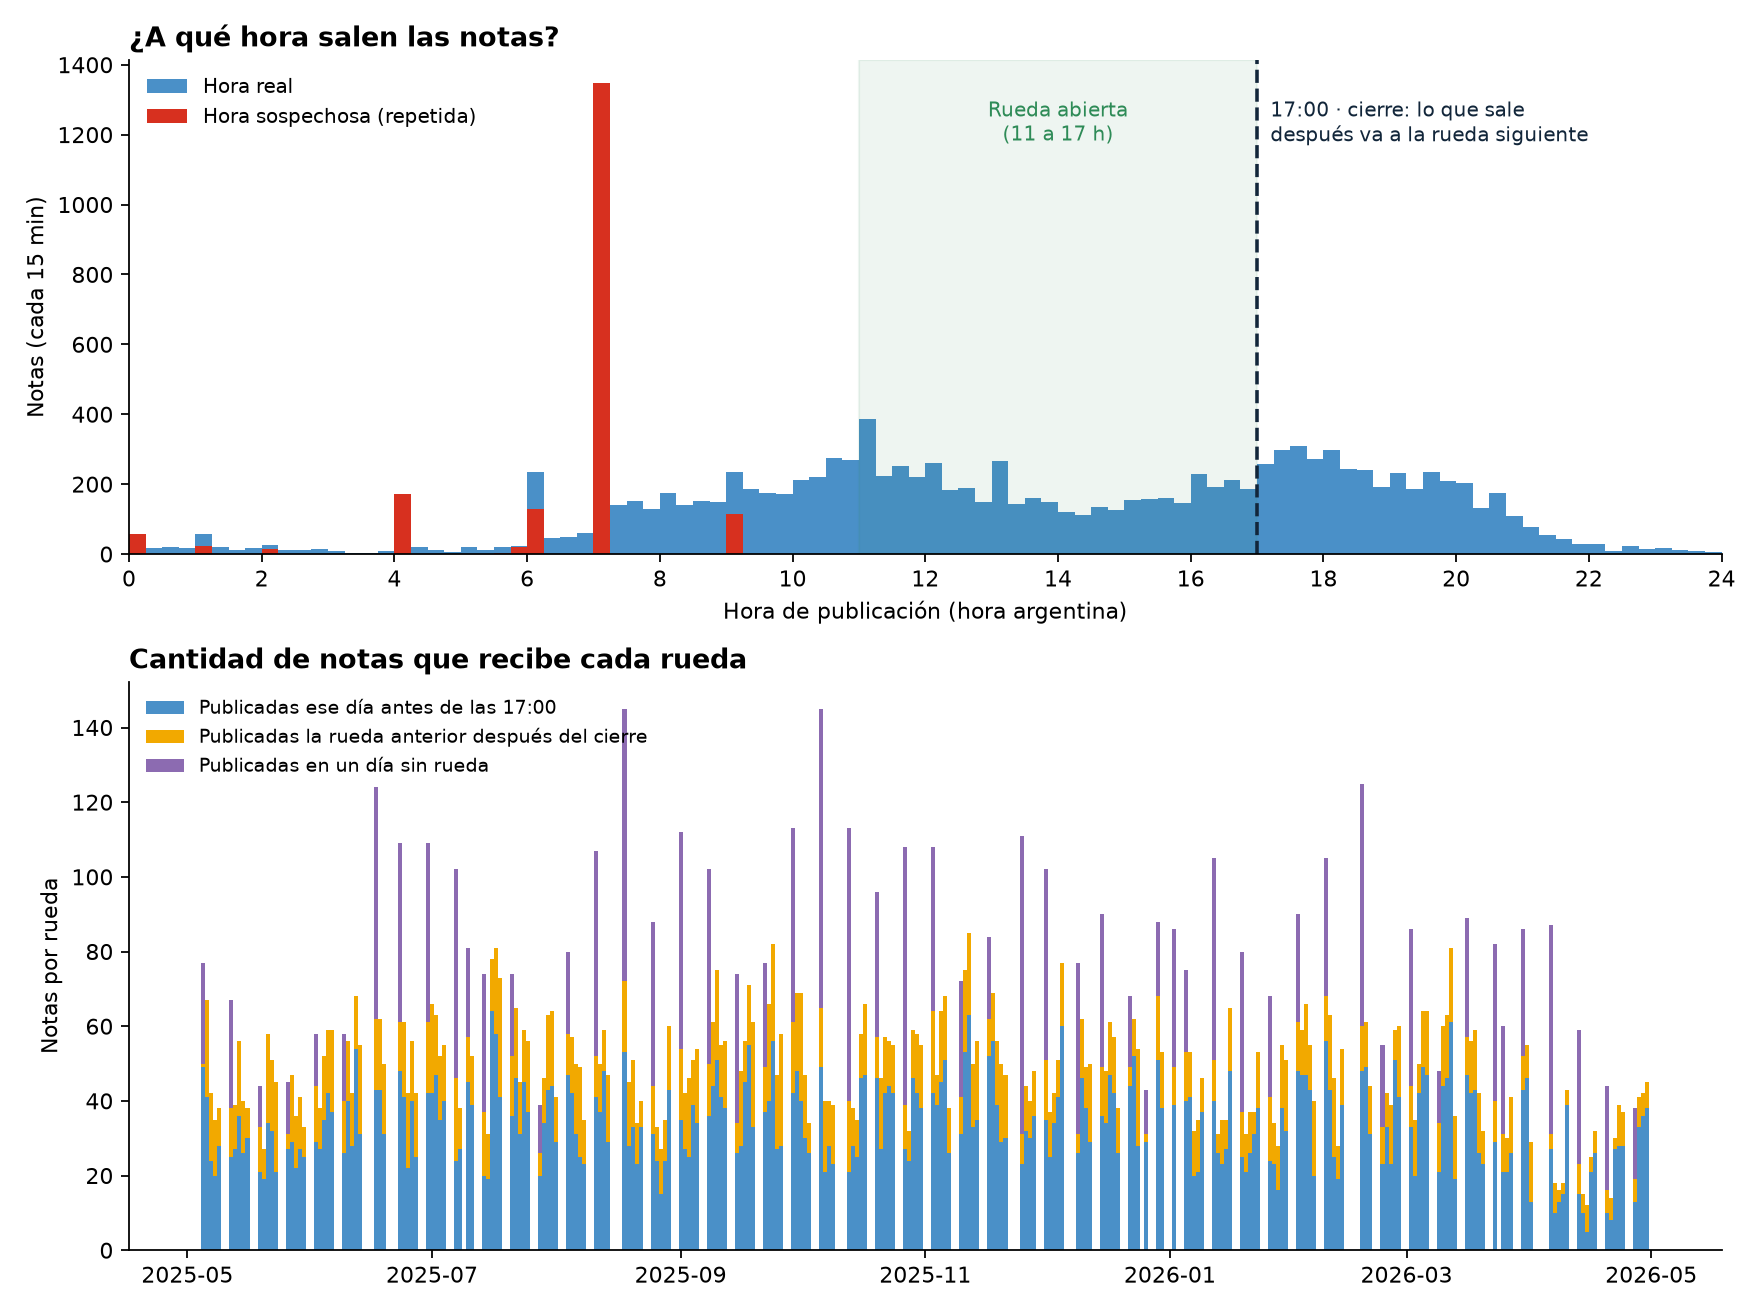
\includegraphics[width=0.76\linewidth]{u1_alineacion_reducida.png}
\caption{Arriba: hora de publicación de las notas, con la rueda sombreada y el cierre de las
17:00; en rojo, horas repetidas que no pueden ser reales. Abajo: notas que recibe cada rueda,
según de dónde vienen. Fuente: elaboración propia (\carpeta{Unión/01_alineacion_noticias_ruedas}).}
\label{fig:u1}
\end{figure}

\textbf{Horas sospechosas.} El 13,4\% de las notas (1.881) tiene una hora que se repite
demasiado dentro de su portal —más del 3\% de sus notas a un mismo minuto—, como las 07:00 de
Clarín o las 00:00 de Ámbito. No es la hora real sino una hora por defecto del sitio. Esas
notas se marcaron y los resultados se repitieron sin ellas (sección~\ref{sec:var-robustez}). La
alineación pasó 10 controles automáticos: por ejemplo, ninguna nota va a una rueda anterior a su
publicación, y ninguna publicada tras el cierre queda en la rueda del mismo día.

\textbf{Límites del instrumento.} La cobertura depende de qué capturó la Wayback Machine y de
la retención de los mapas del sitio; abril de 2026 tiene un hueco de recolección en
iProfesional, el portal más grande, y se marcó para analizarlo aparte. Las notas pertenecen a
sus medios y se usaron únicamente con fines académicos: el análisis trabaja con medidas
agregadas (tono, cantidad, menciones) y no reproduce las notas.
